\section{Detection}
The detection task is the task that the robot will execute whenever it reaches its goal position. During such a task the robot needs to identify the position of the circular tables inside the map. 
To solve this task, we used the data coming from the laser sensor (topic /scan). So, given those data we develop an algorithm that can be summarized with the following steps :
\begin{itemize}
    \item classify points detected by the laser into two different classes :
    \begin{itemize}
        \item circular tables points 
        \item not circular table points (i.e. points of walls, bookshelves etc..)
    \end{itemize}
\end{itemize}
\subsection{Classification of the points}
The first step of the detection algorithm was developed by adapting an obstacle extraction~\cite{detection-and-tracking-2d-geometric-obstacles-from-lrf-data} algorithm that is able to find straight lines and circles. 
In particular, this algorithm consists of :
\begin{itemize}
    \item Grouping points : this step consists of grouping points in order to provide a collection of subsets \(S_{j}\)  representing possibly separate objects. A point \(\vec{p}_{i}\) is assigned to the group of point \(\vec{p}_{i-1}\) if the following criterion is satisfied : \(d_{i-1}^{i} < d_{group} + R_{i}d_{p}\) where :
    \begin{itemize}
        \item \(d_{i-1}^{i}\) is the euclidean distance between point \(\vec{p}_{i}\) and \(\vec{p}_{i-1}\)
        \item \(d_{group}\) is a user defined threshold for grouping
        \item \(R_{i}\) is the length of the vector formed by connecting the origin and point \(\vec{p}_{i}\)
        \item \(d_{p}\) is the angle of increment of the laser sensor
    \end{itemize}
    \begin{center}
        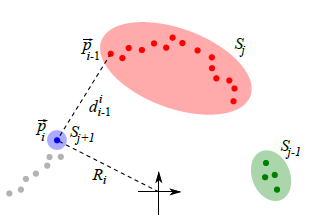
\includegraphics[scale=0.5]{images/detection/grouping-points.png}    
    \end{center}    
    \item Splitting points : in this phase each subset \(S_{j}\) of points is examined only if it contains a number of points greater than \(N_{min}\) points. Moreover, in this step, an Iterative End Point Fit algorithm is used in order to build a leading line upon two extremes points of the group and seeks the point of the group, farthest apart from this line, that is used for splitting the subset. The criterion of splitting two sets in two is the following : \(\bar{d}_{j} > d_{split} + R_{j}d_{p}\) where :
    \begin{itemize}
        \item \(\bar{d}_{j}\) is the distance between the leading line and the farthest point of set \(S_{j}\)
        \item \(d_{split}\) is a user defined threshold for splitting 
        \item \(R_{j}\) is the length of the vector formed by connecting the origin and the farthest point in \(S_{j}\)
        \item \(d_{p}\) is the angle of increment of the laser sensor
    \end{itemize}
    Notice that this procedure is repeated recursively for each new subset until no more splitting occurs. Furthermore, in case of splitting, the point of division is assigned to both the new subsets.
    \begin{center}
        \begin{figure}[H]
            \begin{minipage}{0.5\textwidth}
                \centering
                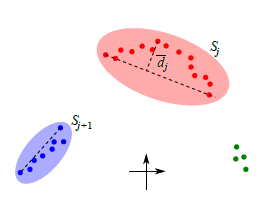
\includegraphics[scale=0.75]{images/detection/splitting-points-before.png}
                \caption{Before Splitting}
            \end{minipage}
            \begin{minipage}{0.5\textwidth}
                \centering
                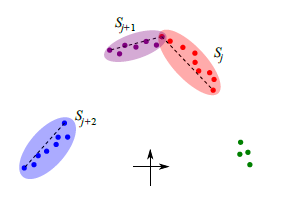
\includegraphics[scale=0.75]{images/detection/splitting-points-after.png}
                \caption{After Splitting}
            \end{minipage}
        \end{figure}            
    \end{center}    
    \item Segmentation : In this step given a subset \(S_{m}\) of points, it is approximated with a segment. This segment is built by using this equation : \(A_{m}x + B_{m}y + C_{m} = 0\) which is fitted by using least square regression to compute the parameters.
    \item Segments merge :  in this phase, given the collection of extracted segments, they are subject to a merging procedure that is composed of two parts : 
    \begin{itemize}
        \item connectivity test : checks if both segments are close to each other by comparing \(d_{0} < d_{merge}\) where :
        \begin{itemize}
            \item \(d_{0}\) denotes the distance between neighboring points of both segments
            \item \(d_{merge}\) is a user defined threshold for connectivity
        \end{itemize}
        \item spread test : checks if both segments are collinear with the following test : \(max (d_{1},d_{2},d_{3},d_{4})  < d_{spread}\) where :
        \begin{itemize}
            \item \(d_{1-4}\) are distances between segments extreme points and the new leading line
            \item \(d_{spread}\) is a user defined threshold for spread
        \end{itemize}
    \end{itemize}
    \begin{center}
        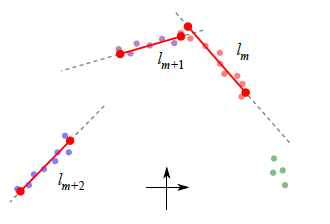
\includegraphics[scale=0.75]{images/detection/segment-points.png}    
    \end{center}  
    \item Circles extraction : in this step, given the set of previous segments detected, we construct for each one of them a equilateral triangle with base equal to the segment and central point away from the origin. Next, on the basis of the triangle we construct an circumscribed circle \(c_{n}\) with radius : \(r_{n} = \frac{\sqrt{3}}{3} \bar{l}_{n}\) (\(\bar{l}_{n}\) is the length of the segment) and central point : \(\vec{p}_{0n} = \frac{1}{2} (\vec{p}_{1n} + \vec{p}_{2n} - \vec{p}_{3n})\). Finally, the radius is enlarged by a user defined threshold \(r_{d}\) and if the resulting radius after enlargement is not greater than another user defined threshold \(r_{max}\) then the circle is added to the set of circles.
    \begin{center}
        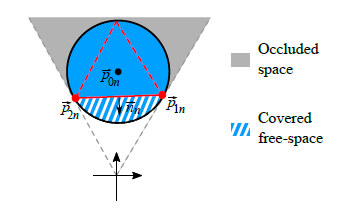
\includegraphics[scale=0.75]{images/detection/circle-extraction.png}    
    \end{center}  
    \item Circles merge : in this phase, given the circles detected in the previous phase, is subject to a merging procedure in order to merge two circle that intersect each other and are very close.   
    \begin{center}
        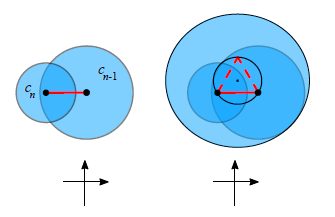
\includegraphics[scale=0.75]{images/detection/circle-merging.png}    
    \end{center}  
\end{itemize}
So, after adapting the code, we were able to find lines and circles given the data provided with the Laser Range Finder. 
\newline
Finally, we return the center of the circles as final position of the objects. 
Notice that, points are computed by rotating the axis as shown in the \textbf{Narrow Passages} section, but, at the end we return the position of the centers of the circular tables in the original reference frame of the robot (not rotated).
